\documentclass{beamer}
\usepackage[utf8]{inputenc}
\usepackage{graphicx}
\usepackage{tabularx}
\usepackage[backend=biber, style=verbose]{biblatex}
\addbibresource{references.bib}


\title{Presentation of Potential of artificial intelligence in reducing energy and carbon emissions of commercial buildings at scale}
\author{Dwayne Mark (Dwayne) Acosta \\ Mohamed Amine Benaziza \\ David Franz \\ Ray Marange \\ James Thompson}
\date{\today}

\begin{document}

\frame{\titlepage}

\begin{frame}{Introduction}
\framesubtitle{Presented by: Ray Marange}
Climate change is accelerating, and buildings are a major contributor, responsible for 39\% of U.S. primary energy use. With urbanization surging and building stock/demand expected to double by 2060, improving building efficiency is no longer optional but urgent.
While AI has transformed industries such as healthcare and finance, its potential in building energy efficiency remains underexplored. AI demonstrates significant potential to reduce costs, enhance benefits, and improve safety across the building lifecycle. The study investigates how AI can reduce energy consumption and carbon emissions in medium-sized office buildings, offering a scalable framework that could be applied globally.
We will explore four key areas: \textbf{Results}, \textbf{Discussion}, \textbf{Methods}, and \textbf{Takeaways \& Reflections}. The study focuses on medium-sized offices, and the results can be extrapolated to offices of any size.
\end{frame}

\begin{frame}{Results part 1}
\framesubtitle{Presented by: Dwayne Mark Acosta}
\begin{itemize}
    \item According to the 2012 U.S. Energy Information Association (EIA), office buildings account for 20\% of commercial energy use.
    \item Median Energy Use Intensity (EUI) of typical office buildings: \textbf{167~kWh/m\textsuperscript{2}} (\textit{EUI\textsubscript{base}}).
    \item Verified low-energy office buildings (\textit{EUI\textsubscript{HEEB}}) achieve: \textbf{57~kWh/m\textsuperscript{2}}.
    \item This yields a Technical Energy Efficiency Saving (TEES) of: \textbf{110~kWh/m\textsuperscript{2}}.
    \item TEES is broken into four key optimization categories:
    \begin{enumerate}
        \item Equipment efficiency
        \item Occupancy influence
        \item Control and operation
        \item Design and construction
    \end{enumerate}
\end{itemize}
\end{frame}

\begin{frame}{Results Part 1}
\framesubtitle{Presented by: Dwayne Mark Acosta}

\begin{itemize}
    \item Medium office buildings make up \textbf{70\%} of total U.S. office energy consumption.
    \item The study used DOE's EnergyPlus tool, based on ASHRAE 90.1, to simulate annual energy use.
    \item Simulations covered four U.S. climate zones (1A, 3B, 4A, 5A) using representative cities.
    \item Natural gas was assumed for heating and hot water, electricity for all other loads.
    \item A total of \textbf{23 improvement cases} were modeled:
    \begin{itemize}
        \item 8 cases for equipment efficiency
        \item 9 cases for design and construction
        \item 6 cases for occupancy behavior and control
    \end{itemize}
\end{itemize}
\end{frame}

\begin{frame}{Results Part 1 – Equipment Efficiency}
    \framesubtitle{Presented by: Dwayne Mark Acosta}
    
    \scriptsize
    \begin{table}[h]
    \centering
    \caption{Equipment Efficiency Improvement Cases}
    \resizebox{\linewidth}{!}{
    \begin{tabularx}{\linewidth}{|c|X|X|}
    \hline
    \textbf{Case} & \textbf{Improvements} & \textbf{Adjustments} \\
    \hline
    E1 & HVAC – Cooling & +20\% \\
    E2 & HVAC – Heating & +12\% \\
    E3 & HVAC – Cases E1 and E2 & +20\%, +12\% \\
    E4 & Lighting – Power density (LPD) & -15\% \\
    E5 & Lighting – Power density (LPD) & -21\% \\
    E6 & Equipment – Power density (EPD) & -10\% \\
    E7 & Equipment – Power density (EPD) & -20\% \\
    E8 & Combined – Cases E1–E7 & \\
    E9 & Case E8 + Heat Pump for space heating & \\
    \hline
    \end{tabularx}
    }
    \end{table}
    \end{frame}

\begin{frame}{Results Part 2 – Design and Construction}
    \framesubtitle{Presented by: Dwayne Mark Acosta}
    
    \scriptsize
    \begin{table}[h]
    \centering
    \caption{Design and Construction Improvement Cases}
    \resizebox{\linewidth}{!}{
    \begin{tabularx}{\linewidth}{|c|X|X|}
    \hline
    \textbf{Case} & \textbf{Improvements} & \textbf{Adjustments} \\
    \hline
    D1 & Orientation & East (90° rotation) \\
    D2 & Orientation & South (180° rotation) \\
    D3 & Orientation & West (270° rotation) \\
    D4 & Envelope (walls, slabs, roofs, windows) & High insulation \\
    D5 & Envelope (walls, slabs, roofs, windows) & Increased infiltration (~60\%) \\
    D6 & Window-to-wall ratio (WWR) & Variation 1 \\
    D7 & Window-to-wall ratio (WWR) & Variation 2 \\
    D8 & Window-to-wall ratio (WWR) & Variation 3 \\
    D9 & Combined – Orientation, insulation, WWR & \\
    \hline
    \end{tabularx}
    }
    \end{table}
    \end{frame}

\begin{frame}{Results Part 3 – Occupant Behavior and Control}
    \framesubtitle{Presented by: Dwayne Mark Acosta}
    
    \scriptsize
    \begin{table}[h]
    \centering
    \caption{Occupant Behavior and Control Improvement Cases}
    \resizebox{\linewidth}{!}{
    \begin{tabularx}{\linewidth}{|c|X|X|}
    \hline
    \textbf{Case} & \textbf{Improvements} & \textbf{Adjustments} \\
    \hline
    B1 & Ventilation control & Open/close windows \\
    B2 & Lighting use & Switch on/off lights \\
    B3 & Electricity consumption & Turn off plug loads \\
    B4 & Lighting use & Dim lights \\
    B5 & HVAC & Turn on/off HVAC systems \\
    B6 & Thermostat & Adjust thermostat settings \\
    \hline
    \end{tabularx}
    }
    \vspace{0.5em}
    \textbf{Estimated Energy Savings:}
    \begin{itemize}
        \item Equipment: 11.5--17.3\%
        \item Design and Construction: 5.9--9.1\%
        \item Occupancy and Control: 15--20\%
    \end{itemize}
    \end{table}
    \end{frame}


\begin{frame}{Integrated Technical Energy-Saving Potential}
    \framesubtitle{Presented by: Dwayne Mark Acosta}
    
    \begin{figure}
        \centering
        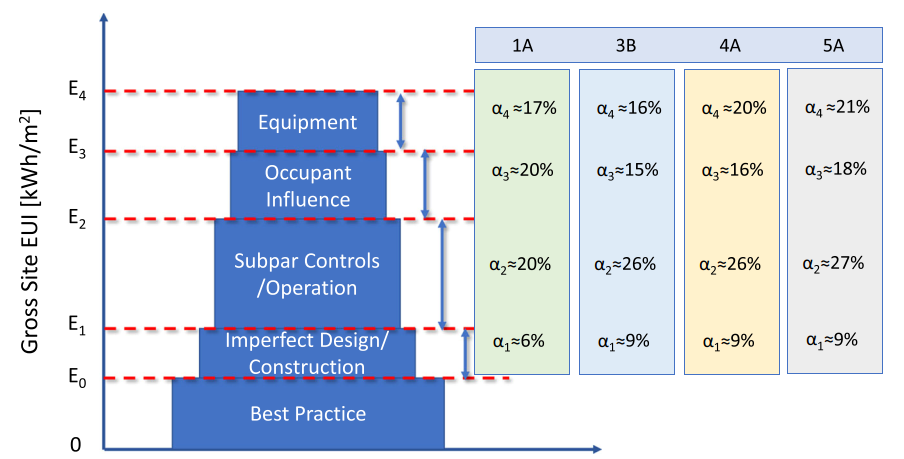
\includegraphics[width=0.95\textwidth]{figures/Integrated technical building energy-saving potential of a typical medium office building in the United States.png}
        \caption{Energy-saving potential by category across U.S. climate zones.}
        \label{fig:category-breakdown}
    \end{figure}
    \end{frame}
    

\begin{frame}{Results part 2}
\framesubtitle{Presented by: David Franz}


\end{frame}

\begin{frame}{Discussions}
\framesubtitle{Presented by: Mohamed Amine Benaziza}

% Just demonstrating what it would looke like for Anime to get a feel for latex syntax.
Method and Scope
\begin{itemize}
    \item Uses engineering + energy-simulation rather than one specific AI technology to estimate how AI can boost building-energy efficiency and cut carbon.
    \item The paper focuses on a medium-office as an example, yet methodology is transferable to other commercial buildings with adjustments.
\end{itemize}
\pause % This means that it will render this slide with the bits above first and then the bits below will appear after going to the next slide. You can add as many as you want. but for lists you can use a special thing below.
Why AI helps
\begin{itemize}[<+->] % Checkout the pdf presentation the list appears incrementally.
    \item Data-driven modeling can tailor solutions and lower costs, accelerating adoption of high-efficiency / net-zero-energy buildings (HEEBs \& NZEBs).
    \item Advanced control models (deep learning, reinforcement learning) could refine accuracy in future work.
\end{itemize}

\end{frame}

\begin{frame}{Methods}
\framesubtitle{Presented by: James Thompson}

\end{frame}
\end{document}
